\section{Evaluations}

% TODO: update this data
\begin{table}
\centering
\caption{Speculative Attack Results}
\label{tab:spec-attack-results}
\begin{tabular}{@{} *4l @{}} \toprule
    &                        & \multicolumn{2}{l}{Bytes per Second} \\
    Attack                  & Cycles for Secret Byte &           100MHz &   3.2GHz \\ \midrule
    Bounds Check Bypass     &                ~884485 &          113 bps & 3618 bps \\
    Branch Target Injection &                ~876602 &          114 bps & 3650 bps \\ \bottomrule
\end{tabular}
\end{table}

\begin{table}
\centering
\caption{BOOM Core Parameters}
\label{tab:boom-core-params}
\begin{tabular}{@{} *2l @{}} \toprule
    Parameter                    & Value \\ \midrule
    Fetch Width                  & 2 \\
    Decode Width                 & 2 \\
    Issue Width                  & 4 \\
    ROB Size                     & 100 \\ \midrule
    L1 Sets                      & 64 \\
    L1 Ways                      & 8 \\
    L1 Linesize                  & 64 bytes \\ \midrule
    BTB Sets                     & 512 \\
    BTB Banks                    & 2 \\
    BTB Ways                     & 4 \\ \midrule
    GShare History Bits          & 23 \\
    GShare Counter Table Entries & 4096 \\ \bottomrule
\end{tabular}
\end{table}

\begin{table}
\centering
\caption{Attack Parameters}
\label{tab:attack-params}
\begin{tabular}{@{} *2l @{}} \toprule
    Parameter                    & Value \\ \midrule
    Cache Hit Threshold          & 50 cycles \\
    Amount of runs on same byte  & 10 rounds \\
    Training rounds for BPU      & 6 training rounds \\
    Cache flush hits on same set & 4 * L1\_WAYS \\
    GShare Counter Table Entries & 4096 \\ \bottomrule
\end{tabular}
\end{table} 

% TODO: updated behavior
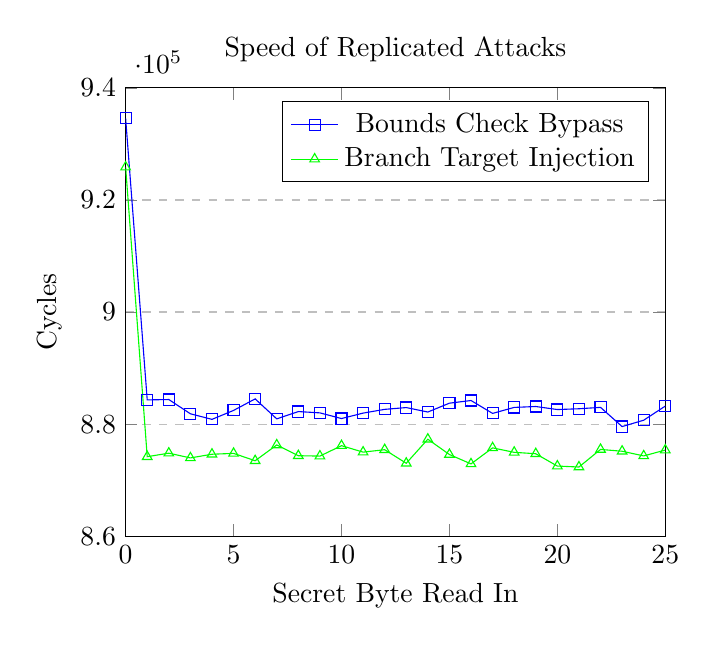
\begin{tikzpicture}
\begin{axis}[
    title={Speed of Replicated Attacks},
    ylabel={Cycles},
    xlabel={Secret Byte Read In},
    xmin=0, xmax=25,
    ymin=860000, ymax=940000,
    legend pos=north east,
    ymajorgrids=true,
    grid style=dashed
]

\addplot[
    color=blue,
    mark=square,
]
coordinates {
    (0 ,934580)
    (1 ,884322)
    (2 ,884387)
    (3 ,881845)
    (4 ,880847)
    (5 ,882446)
    (6 ,884498)
    (7 ,880939)
    (8 ,882241)
    (9 ,882006)
    (10,880994)
    (11,881965)
    (12,882634)
    (13,882954)
    (14,882156)
    (15,883738)
    (16,884212)
    (17,881912)
    (18,882980)
    (19,883142)
    (20,882600)
    (21,882739)
    (22,882989)
    (23,879563)
    (24,880698)
    (25,883218)
};
        
\addplot[
    color=green,
    mark=triangle,
]
coordinates {
    (0 ,925862)
    (1 ,874188)
    (2 ,874815)
    (3 ,873968)
    (4 ,874626)
    (5 ,874778)
    (6 ,873466)
    (7 ,876281)
    (8 ,874361)
    (9 ,874297)
    (10,876153)
    (11,875000)
    (12,875435)
    (13,873015)
    (14,877303)
    (15,874572)
    (16,872902)
    (17,875761)
    (18,874966)
    (19,874715)
    (20,872514)
    (21,872346)
    (22,875481)
    (23,875161)
    (24,874325)
    (25,875371)
};
\legend{Bounds Check Bypass,Branch Target Injection}

\end{axis}
\end{tikzpicture}

\subsection{Base Core Parameters}

The two different attacks were replicated on the BOOM core with the parameters given
in \ref{tab:boom-core-params}. All attacks were measured using FireSim, an open-source
cycle-accurate, FPGA-accelerated scale-out computer system simulation platform [?].

\subsection{Replicating Speculative Attacks}

Overall, the attacks chosen were replicated successfully on the BOOM microarchitecture. A printout
demonstrating leakage of secret information with the Bounds Check Bypass attack
is shown in \ref{ref:spec-attack-printout}. Initial results of the replications
are promising with [FILL IN DATA SENTENCE]. \ref{tab:spec-attack-results}
shows the results of the two attacks. These measurements take into account the clearing
of the tally array before each run, the multiple rounds of training for the BPU,
the single attack run on the victim, and the time to measure out the secret from the attacker array.
The cycle times are close to each other because the code shares a similar structure. The main
differences are around the setup of the {\tt fdiv} manipulation
and the extra arithmetic in the Branch Target Injection attack where you have to calculate
both the index and the address for accessing the function and passing the input. 

\begin{lstlisting}[style=column-code, caption=Printout of Bounds Check Bypass Attack]
want(!) =?= 1.(!) 2.(^A)
want(") =?= 1.(") 2.(^A)
want(#) =?= 1.(#) 2.( C)
want(T) =?= 1.(T) 2.(^A)
want(h) =?= 1.(h) 2.(i)
want(i) =?= 1.(i) 2.(>)
want(s) =?= 1.(s) 2.(^D)
want(I) =?= 1.(I) 2.(^D)
want(s) =?= 1.(s) 2.( ^L)
want(T) =?= 1.(T) 2.(Ò)
want(h) =?= 1.(h) 2.(^F)
want(e) =?= 1.(e) 2.()
want(B) =?= 1.(B) 2.(<9f>)
want(a) =?= 1.(a) 2.(^B)
want(b) =?= 1.(b) 2.(^A)
want(y) =?= 1.(y) 2.()
want(B) =?= 1.(B) 2.(¡)
want(o) =?= 1.(o) 2.(^H)
want(o) =?= 1.(o) 2.(4)
want(m) =?= 1.(m) 2.(k)
want(e) =?= 1.(e) 2.(^C)
want(r) =?= 1.(r) 2.(^A)
want(T) =?= 1.(T) 2.(^C)
want(e) =?= 1.(e) 2.(^O)
want(s) =?= 1.(s) 2.(^D)
want(t) =?= 1.(t) 2.(^A)
\end{lstlisting}\label{ref:spec-attack-printout}

\subsection{Spec Buffer}
